%\documentclass[compress,notesonly]{beamer} %compress to make bars as small as possible
                                           %notesonly to add note not visible on screen (\note[]{})
%\documentclass[compress,slidescentered,notes=show]{beamer}
\documentclass[compress,slidescentered,notes=hide]{beamer}

%---------------FONT AND LANGUAGES ---------------------------
\usepackage[utf8]{inputenc}
%\usepackage[T1]{fontenc}
\usepackage[english]{babel}
\usepackage{pifont}

%--------------FORM ------------------------------
%\usepackage{beamerthemesplit}
\usepackage{multicol} %possibility to create columns
\usepackage{comment} 
%\usepackage[absolute,showboxes, overlay]{textpos}
%\textblockorigin{1mm}{1mm}
%\TPshowboxestrue % or false to display contour
\usepackage{array}
\pdfpageattr {/Group << /S /Transparency /I true /CS /DeviceRGB>>}
\usenavigationsymbolstemplate{}

\usetheme{Darmstadt} %Frankfurt} 
%\useoutertheme{smoothbars} %to add numerotation
\usepackage{color} %creation of own colors
%\useoutertheme{infolines} %to add numerotation
%%\usecolortheme[named=SeaGreen]{structure}
\definecolor{bleuclair}{rgb}{0.2,0.9,0.8}
%%\definecolor{mycyan}{rgb}{.19,0.5,0.5}
\definecolor{mycyan}{rgb}{0.2,0.6,0.6}
\setbeamercolor*{palette primary}{use=structure,fg=white,bg=mycyan}
\setbeamercolor{block title}{bg=mycyan,fg=black}%bg=background, fg= foreground
\setbeamercolor{block body}{bg=lightgray,fg=black}%bg=background, fg= foreground
\setbeamercolor{structure}{bg=black, fg=mycyan}
\setbeamercolor{normal text}{fg=black}
\setbeamercolor{alerted text}{fg=red}
\setbeamercolor{frametitle}{fg=white}
\setbeamercolor{title}{fg=black}
\setbeamercolor{titlelike}{fg=black}
\setbeamercolor{title}{fg=black}
\setbeamercolor{section in sidebar}{fg=black}
\setbeamercolor{section in sidebar shaded}{fg=gray}
\setbeamercolor{subsection in sidebar}{fg=black}
\setbeamercolor{subsection in sidebar shaded}{fg=gray}
\setbeamercolor{itemize item}{fg=mycyan}
\setbeamercolor{section in tableofcontents}{fg=black,bg=black}
\setbeamercolor{part title shaded}{bg=mycyan!50, fg=white}
\setbeamercolor*{item projected}{fg = white, bg=mycyan} 
%\useoutertheme{shadow}
%\setbeamercolor{sidebar}{bg=red}
%\beamertemplatetransparentcovered %set transparancy
\newcommand{\gu}[1]{#1}
%usepackage{default}
\usepackage{geometry} %put margin
\geometry{hmargin=0.25cm, vmargin=0.0cm}
\setbeamersize{text margin left=2mm, text margin right=2mm}
%\setbeamersize{text margin top=0cm}
%\setbeamersize{sidebar width left=0cm}
%\setbeamersize{sidebar width right=0cm}
%\usepackage{fullpage}
\setbeamertemplate{background}{\includegraphics[width=\paperwidth,height=\paperheight]{./pict/slide0006_background.png}}
\setcounter{tocdepth}{3}
%\setbeamertemplate{part page} %To add number to Part 
%{
%  \begin{centering}
%    {\usebeamerfont{part name}\usebeamercolor[fg]{part name}\partname~\insertpartnumber}
%    \vskip1em\par
%    \begin{beamercolorbox}[sep=16pt,center]{part title}
%      \usebeamerfont{part title}\insertpart\par
%    \end{beamercolorbox}
%  \end{centering}
%}
\makeatletter
\AtBeginPart{\beamer@tocsectionnumber=0\relax\c@section=0
%  \addtocontents{toc}{\protect\beamer@partintoc{\the\c@part}{\beamer@partnameshort}{\the\c@page}}
}
%\@addtoreset{part}{section}
\makeatother

%-------------GRAPHICS ----------------------------
\usepackage{graphicx} %add pictures
\graphicspath{{./pict/}{pict_nemo/}{/data2/gaultier/NEMO/DIAG/}} %path to pictures
\usepackage{tikz} %add schemes
\usetikzlibrary{shapes} %add diamonds shape to schemes
\usepackage{multimedia} %add video
\usepackage{array}
\pdfpageattr {/Group << /S /Transparency /I true /CS /DeviceRGB>>} %avoid color troubles using eps and acroread
\renewcommand{\figurename}{Fig.}
\setlength{\unitlength}{1cm} %to use pictures
\newcommand{\ftitle}[1]{\begin{center}\textcolor{mycyan}{#1} \end{center}} %title for figures
\newcommand{\legende}[1]{\textit{\footnotesize #1}}
\newcommand{\mypart}[1]{\begin{beamercolorbox}[sep=3pt,center, rounded=true]{part title}
                       \usebeamerfont{part title} #1 \par
                       \end{beamercolorbox}}
\newcommand{\myspart}[1]{\begin{beamercolorbox}[sep=3pt,center, rounded=true]{part title shaded}
                       \usebeamerfont{part title} #1 \par
                       \end{beamercolorbox}}



%------------MAKE TITLE ----------------------------
\title{On the joint use of high resolution tracer images \hspace{4cm} and altimetric data for the control of ocean circulations.}
%\subtitle{\vspace{1.5em} \textbf{A Data Assimilation strategy}}
\author[S\'eminaire LPO]{Lucile Gaultier, Jacques Verron, Pierre Brasseur, Jean-Michel Brankart}
\date{\textit{February 15, 2013}}

%\logo{\includegraphics[height=1.5cm]{./pict/logo_meom.jpeg}}
%\logo{\insertframenumber/\inserttotalframenumber}
%\pgfdeclareimage[height=1.2cm]{legi}{./pict/logo_legi.jpeg}
%\logo{\pgfuseimage{legi}}

\begin{document}

%1%%%%%%%%%%%%%%%%%%%%%%%%%%%%%%%%%%%%%%%%%%%%%%%%%%%%%%%%%%%%%%%%%%%%%
\begin{frame}
  \maketitle
\setbeamercolor*{palette primary}{use=structure,fg=white,bg=bleuclair}
  \begin{center}
    \includegraphics[height=1.3cm]{./pict/logo/logo_meom.jpeg}
    \hspace{0.5cm}
    \includegraphics[height=1.3cm]{./pict/logo/logo_lgge.jpeg}
    \hspace{0.5cm}
    \includegraphics[height=1.3cm]{./pict/logo/logo_cnrs.jpeg}
    \hspace{0.5cm}
    \includegraphics[height=1.3cm]{./pict/logo/logo_cnes.jpeg}
  \end{center}
  \note{
}
\end{frame}
%%%%%%%%%%%%%%%%%%%%%%%%%%%%%%%%%%%%%%%%%%%%%%%%%%%%%%%%%%%%%%%%%%%%%%%%

\logo{\textcolor{mycyan}{\insertframenumber/\inserttotalframenumber}}
%%%%%%%%%%%%%%%%%%%%%%%%%%%%%%%%%%%%%%%%%%%%%%%%%%%%%%%%%%%%%%%%%%%%%%%%
\begin{frame}
%  \frametitle{I INTRODUCTION}
  \mypart{I INTRODUCTION}
  \tableofcontents[part=1] %[hideallsubsections]
\end{frame}
%%%%%%%%%%%%%%%%%%%%%%%%%%%%%%%%%%%%%%%%%%%%%%%%%%%%%%%%%%%%%%%%%%%%%%%%
\begin{frame}
  \mypart{II METHOD}
  \tableofcontents[part=2] %[hideallsubsections]
\end{frame}
%%%%%%%%%%%%%%%%%%%%%%%%%%%%%%%%%%%%%%%%%%%%%%%%%%%%%%%%%%%%%%%%%%%%%%%%

%%%%%%%%%%%%%%%%%%%%%%%%%%%%%%%%%%%%%%%%%%%%%%%%%%%%%%%%%%%%%%%%%%%%%%%%
\begin{frame}
%  \frametitle{III RESULTS}
  \mypart{III RESULTS}
  \tableofcontents[part=3] %[hideallsubsections]
\end{frame}
%%%%%%%%%%%%%%%%%%%%%%%%%%%%%%%%%%%%%%%%%%%%%%%%%%%%%%%%%%%%%%%%%%%%%%%%

%-------------------%%
\part{Introduction} %%
%-------------------%%
%%%%%%%%%%%%%%%%%%%%%%%%%%%%%%%%%%%%%%%%%%%%%%%%%%%%%%%%%%%%%%%%%%%%%%%%
\begin{frame}
  \frametitle{\insertromanpartnumber \hspace{1em} \insertpart}
  \mypart{I INTRODUCTION}
  \tableofcontents[hideotherpart]
  \myspart{II METHOD}
  \myspart{III RESULTS}
\end{frame}
%%%%%%%%%%%%%%%%%%%%%%%%%%%%%%%%%%%%%%%%%%%%%%%%%%%%%%%%%%%%%%%%%%%%%%%%

\section{Ingredients of the talk}
%----------------------------------------------------------------------%
        \subsection{Submesoscales}
%%%%%%%%%%%%%%%%%%%%%%%%%%%%%%%%%%%%%%%%%%%%%%%%%%%%%%%%%%%%%%%%%%%%%%%%
\begin{frame}
  \begin{columns}
   \column{.01\textwidth}
    \column{.50\textwidth}
    \begin{block}{}
      \begin{itemize}
        \item Intermediate scale between Mesoscale and dissipative scales.\\
        \item Filaments length: 1-10~km.
      \end{itemize}
    \end{block}
    \begin{block}{}
      Sub-mesoscales generated by mesoscale dynamics \\
      To what extend can sub-mesoscales control mesoscales?
    \end{block}
   \column{.01\textwidth}
    \column{.48\textwidth}
    \includegraphics[width=0.9\linewidth]{./pict/misc/submeso.png}\\
    %\includegraphics[width=0.6\linewidth]{frontogenesis.png}\\ 
     \small{Baroclinic instability in an idealized model (Chlorophyll)}
  \end{columns}
  \begin{block}{Importance of sub-mesoscales }
    %\begin{itemize}
      \ding{226} Impact on larger scale circulation \\
      \ding{226} Energetic importance \\
    %\end{itemize}
     \small{(Capet \& al, 2008, Thomas \& al, 2008, Klein \& al, 2008, Ferrari \& al, 2008)  }
  \end{block}
\note{link between meso and sub-mesoscales. can we contr�le mesoscale dynamics using sub-mesoscales information?}
\end{frame}
%%%%%%%%%%%%%%%%%%%%%%%%%%%%%%%%%%%%%%%%%%%%%%%%%%%%%%%%%%%%%%%%%%%%%%%%

        \subsection{Altimetry}
%%%%%%%%%%%%%%%%%%%%%%%%%%%%%%%%%%%%%%%%%%%%%%%%%%%%%%%%%%%%%%%%%%%%%%%%
\begin{frame}
  \begin{block}{Altimetric data}
  \begin{itemize}
    \item Measure of sea surface height along track
    \item Geostrophic velocity derived from ssh gradients
    \item Data: e.g. AVISO (interpolated maps, velocity, ssh)
  \end{itemize}
  Use of gridded SSH and velocity: interpolation between tracks
  \end{block}
  \begin{minipage}{0.49\textwidth}
  \begin{figure}
    \includegraphics[width=0.6\linewidth]{along_track_tas.png} \\
    {\small Jason and Envisat tracks, 15 days before and after December 22, 2004, Tasmania }
  \end{figure}
  \end{minipage}
  \begin{minipage}{0.49\textwidth}
  \begin{block}{}
    \ding{226} 3 satellites are necessary to capture mesoscale signal (Morrow and Le Traon, 2011).\\
    \ding{226} Sub-mesoscales cannot currently be seen by altimetric satellites (Fu and Ferrari, 2008).
  \end{block}
  \end{minipage}
\note{Enhance the fact that Altimetric product are a rough estimation of the dynamics, lost of information during the process. }
\end{frame}
%%%%%%%%%%%%%%%%%%%%%%%%%%%%%%%%%%%%%%%%%%%%%%%%%%%%%%%%%%%%%%%%%%%%%%%%

        \subsection{Tracer}
%%%%%%%%%%%%%%%%%%%%%%%%%%%%%%%%%%%%%%%%%%%%%%%%%%%%%%%%%%%%%%%%%%%%%%%%
\begin{frame}
  \begin{block}{Interested in tracers visible from space}
  \begin{itemize}
     \item Sea Surface Temperature (near IR, visible)
     \item Ocean Color: Chlorophyll (visible)
  \end{itemize}
  \end{block}
  \begin{minipage}{0.49\textwidth}
    \includegraphics[width=0.9\linewidth]{./pict/sstbret.png}\\
    {\small SST from MODIS sensor \\ (4-11 August 2012)}
  \end{minipage}
  \begin{minipage}{0.49\textwidth}
    \includegraphics[width=0.9\linewidth]{./pict/chlbret.png}\\
   {\small Chlorophyll from MODIS sensor \\ (4-11 August 2012)}
  \end{minipage}
  \begin{block}{}
  Sub-mesoscales filaments revealed by tracer images
  \end{block}
\end{frame}
%%%%%%%%%%%%%%%%%%%%%%%%%%%%%%%%%%%%%%%%%%%%%%%%%%%%%%%%%%%%%%%%%%%%%%%%

  \subsection{FSLE}
%%%%%%%%%%%%%%%%%%%%%%%%%%%%%%%%%%%%%%%%%%%%%%%%%%%%%%%%%%%%%%%%%%%%%%%%
\begin{frame}
  \frametitle{FSLE: Finite-Size Lyapunov Exponents}
  \begin{block}{}
   Tracer observation and FSLE derived from altimetric velocity have shown similar patterns (Lehahn \& al 2008, d'Ovidio \& al 2004).
  \end{block}
  \begin{columns}
    \begin{column}{0.49\textwidth}
      \begin{figure}
        \includegraphics[width=4.9cm]{./pict/misc/lohafex.png}
      \end{figure}
      \legende{Chlorophyll, South Atlantic, d'Ovidio \& al, 2004}
    \end{column}
    \begin{column}{0.49\textwidth}
      \begin{figure}
        \includegraphics[width=4.9cm]{./pict/misc/lehahn.png}
      \end{figure}
      \legende{Chlorophyll, Pomme area, Lehahn \& al, 2008}
    \end{column}
  \end{columns}
\end{frame}
%%%%%%%%%%%%%%%%%%%%%%%%%%%%%%%%%%%%%%%%%%%%%%%%%%%%%%%%%%%%%%%%%%%%%%%%
   
     \subsection{Data Assimilation}
%%%%%%%%%%%%%%%%%%%%%%%%%%%%%%%%%%%%%%%%%%%%%%%%%%%%%%%%%%%%%%%%%%%%%%%%
\begin{frame}
  \begin{block}{}
     Data Assimilation aims at finding an optimal compromise between information of different natures, space and time sampling. \\
     The sources are generally some observations (satellite, in-situ) and a numerical model. \\

  \end{block}
  \begin{figure}
    \includegraphics[width=0.8\linewidth]{pict/misc/brasseur_da.png}
  \end{figure}
  \legende{Conceptual representation of filtering with sequential assimilation, Brasseur,
 2006}
\end{frame}
%%%%%%%%%%%%%%%%%%%%%%%%%%%%%%%%%%%%%%%%%%%%%%%%%%%%%%%%%%%%%%%%%%%%%%%%

%Slide model? model nath+model levy

\section{Motivation}% and objectives}
%----------------------------------------------------------------------%

	\subsection{Observation from space}
%%%%%%%%%%%%%%%%%%%%%%%%%%%%%%%%%%%%%%%%%%%%%%%%%%%%%%%%%%%%%%%%%%%%%%%%
\begin{frame}
 %CAN SUBMESOSCALES CONTROL MESOSCALES? 
  \begin{multicols}{2}
  \begin{minipage}{0.49\textwidth}
%  \begin{columns}
%   \column{0.01\textwidth}
%   \column{0.51\textwidth}
 % \begin{center}
    \includegraphics[width=0.5\linewidth]{along_track_tas.png}\\
    \legende{\small Jason and Envisat tracks, 15 days before and after December 22, 2004, Tasmania }
 % \end{center}
    \begin{block}{}
        Sub-mesoscales are not resolved by altimetry.
 %bservations of the dynamics (altimetry).
    \end{block}
  \end{minipage}
  \begin{minipage}{0.49\textwidth}
%  \column{0.0001\textwidth}
%  \column{0.46\textwidth}
  \begin{center}
    \only<2>{\includegraphics[width=0.61\linewidth]{A2004358041000_L2_LAC_OC.png}\\
\legende{\small Chlorophyll, December 22, 2004, Tasmania }}
%  \end{center} 
  \only<2>{
  \begin{block}{}
     Sub-mesoscales are observed using satellite tracer sensors.
     \vspace{0.20em}
  \end{block}}
  \end{center}
  \end{minipage}
\end{multicols}
%  \column{0.0001\textwidth}
%  \end{columns}
  \only<2>{
  \begin{block}{}
    Joint use of altimetry and high resolution tracer observation to improve the dynamics.
  \end{block}}
\note{
Obs altimetric. Obs image
}
\end{frame}
%%%%%%%%%%%%%%%%%%%%%%%%%%%%%%%%%%%%%%%%%%%%%%%%%%%%%%%%%%%%%%%%%%%%%%%%

\section{Objective and Strategy}
%----------------------------------------------------------------------%

	\subsection{A data assimilation approach}
%%%%%%%%%%%%%%%%%%%%%%%%%%%%%%%%%%%%%%%%%%%%%%%%%%%%%%%%%%%%%%%%%%%%%%%%
\begin{frame}
%\frametitle{Context of the inversion of information}
  \begin{block}{Data Assimilation}
    \ding{226} aims at finding an optimal compromise between information of different natures, space and time sampling.
  \end{block}
  \begin{tikzpicture}
%    \node[color=blue, text width=4cm, text centered] (UV) at (7,2.7) {Mesoscale field};
    \node[color=black, text width=3.9cm, text centered] (pUV) at (7,0) {\includegraphics[width=0.9\linewidth]{aviso_20079_tasmania.png}\\ %};
        \legende{Velocity map}}; %mania region, December 22, 2004}};
%    \node[color=green, text width=4cm, text centered] (TRA) at (0,2.7) {Sub-mesoscale tracer image};
    \node[color=black, text width=3.9cm, text centered] (pTRA) at (0,0) {\includegraphics[width=0.9\linewidth]{pict/A2004358041000_L2_LAC_OC.png}\\ %};
        \legende{Chlorophyll image}}; %, Tasmania region, December 22, 2004}};
    \node[draw] (int) at (3.7,1) {\large{?}};
  \draw[->,>=latex] (pTRA)--(pUV);
    \node[color=black, text width=3.9cm, text centered] (mtext) at (3.5,-1.6) { \legende{Tasmania region,\\ December 22, 2004}};
  \end{tikzpicture}

  \visible<2->{
  \begin{block}{Use of a Data Assimilation approach}
  The inversion of sub-mesoscale tracer information to correct mesoscale velocity has never been done before
  %Optimization problem
  \end{block}}
\note{Add complexity in assimilation to enhance the signal. }
\end{frame}

%\begin{frame}
%Objective
%\end{frame}
%%%%%%%%%%%%%%%%%%%%%%%%%%%%%%%%%%%%%%%%%%%%%%%%%%%%%%%%%%%%%%%%%%%%%%%%

%-----------------------------%%
\part{Methodological aspects} %% 
%-----------------------------%%

\begin{frame}
  \frametitle{\insertromanpartnumber \hspace{1em} \insertpart}
  \myspart{I INTRODUCTION}
  \mypart{II METHOD}
  \tableofcontents[hideotherpart]
  \myspart{III RESULTS}
\end{frame}
%%%%%%%%%%%%%%%%%%%%%%%%%%%%%%%%%%%%%%%%%%%%%%%%%%%%%%%%%%%%%%%%%%%%%%%%

\section{Comparing velocity and tracer images}
%----------------------------------------------------------------------%

%%%%%%%%%%%%%%%%%%%%%%%%%%%%%%%%%%%%%%%%%%%%%%%%%%%%%%%%%%%%%%%%%%%%%%%%
%\begin{frame}
%  \frametitle{Methodoligical aspects}
%  \tableofcontents[hideotherpart,currentsection]
%\end{frame}
%%%%%%%%%%%%%%%%%%%%%%%%%%%%%%%%%%%%%%%%%%%%%%%%%%%%%%%%%%%%%%%%%%%%%%%%

	\subsection{Find a proxy between tracer and velocity}
%%%%%%%%%%%%%%%%%%%%%%%%%%%%%%%%%%%%%%%%%%%%%%%%%%%%%%%%%%%%%%%%%%%%%%%%
\begin{frame}
 %\frametitle{A proxy is needed}
  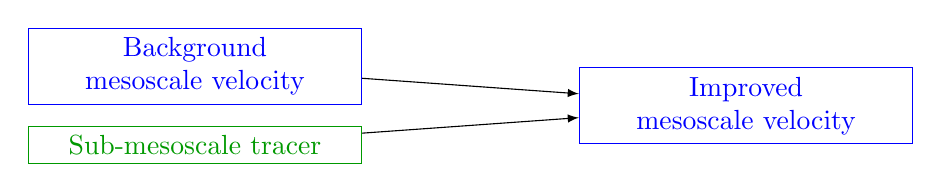
\begin{tikzpicture}
    \node[draw, color=blue, text width=4cm, text centered] (meso) at (0,0) {Background mesoscale velocity};
    \node[draw, color=green!60!black, text width=4cm, text centered](subm) at (0,-1) {Sub-mesoscale tracer};
    \node[draw, color=blue, text width=4cm, text centered] (cor) at (7,-0.5) {Improved mesoscale velocity};
    \draw[->,>=latex] (meso)--(cor);
    \draw[->,>=latex] (subm)--(cor);
  \end{tikzpicture}
  \vspace{0.6cm}
  \begin{block}{Find the correction of this background the most compatible with tracer information}
    \begin{itemize}
     \item The direct measure of the distance between $\vec{\bf{u}}$ and \textbf{Tracer} is not possible
     \item Need to find a go-between variable
     \item Use of Finite-Size Lyapunov Exponents as a proxy (FSLE)
    \end{itemize}
  \end{block}
  %\begin{block}{}
    \small{See Gaultier \& al, 2012 for details}
\end{frame}
%5%%%%%%%%%%%%%%%%%%%%%%%%%%%%%%%%%%%%%%%%%%%%%%%%%%%%%%%%%%%%%%%%%%%%%%
\begin{frame}
  %\frametitle{Physical meaning of Lyapunov Exponents}
  Lyapunov exponents are defined as the exponential rate of separation, averaged over time \\
  \vspace{1cm}
  \centering
  \begin{columns}
    \begin{column}{0.5\textwidth}
       \begin{center}
       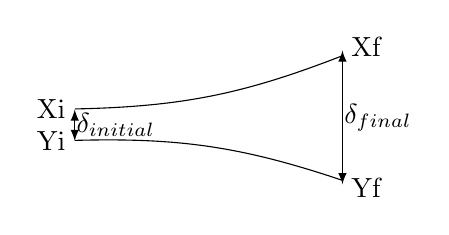
\begin{tikzpicture}
        \node (xi) at (0,0.2) {Xi};
        \node (xf) at (4,1) {Xf};
        \node (yi) at (0,-0.2) {Yi};
        \node (yf) at (4,-0.8) {Yf};
        \node (di) at (0.82,0) {$\delta_{initial}$};
        \node (df) at (4.15,0.1) {$\delta_{final}$};

        \draw[-,>=latex] (xf) to[bend left=10] (xi);
        \draw[-,>=latex] (yf) edge[bend right=10] (yi);
        \draw[<->,>=latex] (0.3,0.2)--(0.3,-0.2);
        \draw[<->,>=latex] (3.7,0.95)--(3.7,-0.75);
      \end{tikzpicture}
      \end{center}
    \end{column}
    \begin{column}{0.49\textwidth}
      \begin{block}{FSLE}
      $\lambda  = \frac{1}{T} \times log(\frac{\delta_{final}}{\delta_{initial}}) $ \\
       Inverse of the time T for particles to be separated from $\delta_{initial}$ to $\delta_{final}$
      \end{block}
%      \vspace{1cm}
%      \legende{Backward (red) and forward (green) integration of trajectories}
    \end{column}
  \end{columns}
 \vspace{1cm}
% Lyapunov exponents constitute Lagrangian transport barriers between different regions (Lehahn \& al (2007)).
  \begin{block}{Lyapunov Exponent constitute Lagrangian transport barriers between different regions}
     Particles are separated by a distance $\delta_{initial}$ \\
     Advect particles backward in time \\
     Record the time T at which one of the distances become larger than $\delta_{final}$
  \end{block}
%  Stable and Unstable Manifolds constitute Lagrangian transport barriers between different regions because they are material invariant curves that cannot be crossed by purely advective process
  \note{Lyapunov exponents are defined as the exponential rate of separation, averaged over time. 
In this study we'll use Finite time Lyapunov Exponent. 
In practical terms we integrate the trajectories of particles and calculate the final distance of two particles, initially at distance delta after a time T. }
\end{frame}
%%%%%%%%%%%%%%%%%%%%%%%%%%%%%%%%%%%%%%%%%%%%%%%%%%%%%%%%%%%%%%%%%%%%%%%%

       \subsection{Consistency of FSLE as a proxy}
%%%%%%%%%%%%%%%%%%%%%%%%%%%%%%%%%%%%%%%%%%%%%%%%%%%%%%%%%%%%%%%%%%%%%%%%
\begin{frame}
%\frametitle{Proxy FSLE consistent}
%The FSLE is our proxy
%What is the FSLE
  \begin{columns}
    \begin{column}{0.5\textwidth}
      \begin{figure}%[!htbp]
        \includegraphics[width=4.5cm]{pict/fsle_24_stat_reg_20814_s_atl.png}\\
        \legende{FSLE, South Atlantic region, \\December 27, 2006}
      \end{figure}
    \end{column}
    \begin{column}{0.5\textwidth}
      \begin{figure}
        \includegraphics[width=4.5cm]{pict/A2006360165000_L2_LAC_SST.png}\\
        \legende{Tracer (SST), South Atlantic region, \\December 27, 2006}
      \end{figure}
    \end{column}
  \end{columns}
  \begin{block}{}
  Lyapunov measures stirring in a fluid \\
  $\rightarrow$ Link between sub-mesoscale dynamics and biologic stirring. \\
  (Lehahn \& al, 2008, d'Ovidio \& al, 2004)
  \end{block}
  \begin{block}{}
  \begin{itemize}
    \item Binarisation of FSLE
    \item Binarisation of the norm of the gradient of tracer filtered image, image processing to reduce the noise (developed by LJK) 
  \end{itemize}
  \end{block}
  %Maximum lines of Lyapunov exponents and frontal tracer structures present similar patterns (d'Ovidio \& al (2004)).
  \note{Roughness of the image processing}
\end{frame}
%%%%%%%%%%%%%%%%%%%%%%%%%%%%%%%%%%%%%%%%%%%%%%%%%%%%%%%%%%%%%%%%%%%%%%%%

\section{Method of Inversion}
%----------------------------------------------------------------------%

%%%%%%%%%%%%%%%%%%%%%%%%%%%%%%%%%%%%%%%%%%%%%%%%%%%%%%%%%%%%%%%%%%%%%%%%
%\begin{frame}
%  \frametitle{Methodoligical aspects}
%  \tableofcontents[hideotherpart,currentsection]
%\end{frame}
%%%%%%%%%%%%%%%%%%%%%%%%%%%%%%%%%%%%%%%%%%%%%%%%%%%%%%%%%%%%%%%%%%%%%%%%

	\subsection{Overview of the method}
%%%%%%%%%%%%%%%%%%%%%%%%%%%%%%%%%%%%%%%%%%%%%%%%%%%%%%%%%%%%%%%%%%%%%%%%
\begin{frame}
%\frametitle{Inversion Method}
 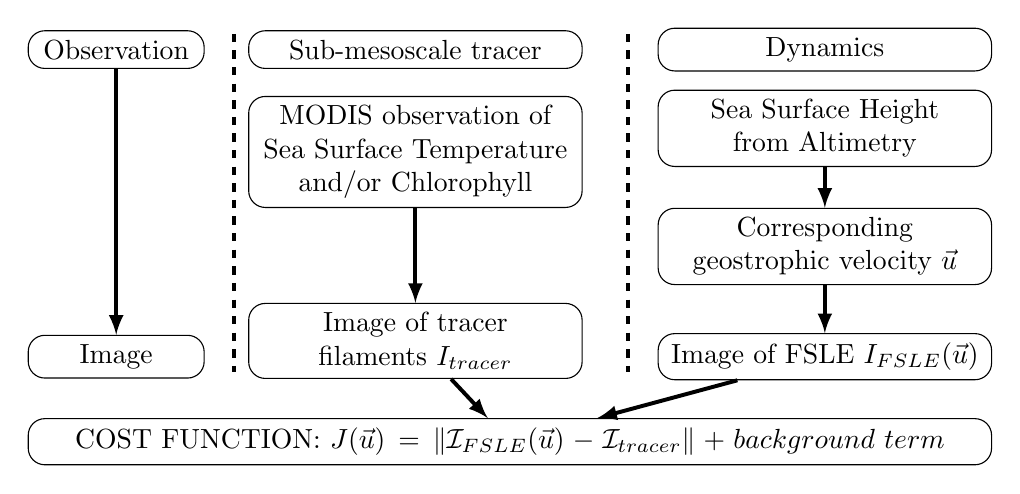
\begin{tikzpicture}
    \tikzset{pname/.style={draw,rectangle,rounded corners=6pt},text centered,color=black}
    \tikzstyle{fleche}=[->,>=latex,line width=0.5mm]
    \node[pname,text width=2cm] (OBS) at (4,8.98) {Observation};
    \node[pname,text width=2cm] (IM) at (4,5.08) {Image};
    \draw[fleche] (OBS)--(IM);
    \draw[dashed,line width=0.5mm] (5.5,9.18)--(5.5,4.88);

    \node[pname,text width=4cm] (TRA) at (7.8,8.98) {Sub-mesoscale tracer};
    \node[pname,text width=4cm] (DYN) at (13,8.98) {Dynamics};
    \draw[dashed,line width=0.5mm] (10.5,9.18)--(10.5,4.88);
    \node[pname,text width=4cm] (OBSTRA) at (7.8,7.68) {MODIS observation of Sea Surface Temperature and/or Chlorophyll};
    \node[pname,text width=4cm] (OBSSSH) at (13,7.98) {Sea Surface Height from Altimetry};
    \node[pname,text width=4cm] (OBSUV) at (13,6.48) {Corresponding geostrophic velocity $\vec{u}$};
    \draw[fleche] (OBSSSH)--(OBSUV);

    \node[pname, text width=4cm] (IMTRA) at (7.8,5.28) {Image of tracer filaments $I_{tracer}$};
    \node[pname,text width=4cm] (IMDYN) at (13,5.08) {Image of FSLE $I_{FSLE}(\vec{u})$};
    \draw[fleche] (OBSTRA)--(IMTRA);
    \draw[fleche] (OBSUV)--(IMDYN);

   \node[pname, text width=12cm] (J) at (9,4.00) {COST FUNCTION: $J(\vec{u})=\|\mathcal{I}_{FSLE}(\vec{u}) -\mathcal{I}_{tracer}\| + background\ term$};
   \draw[fleche] (IMTRA)--(J);
   \draw[fleche] (IMDYN)--(J);
  \end{tikzpicture} \\
\end{frame}
%%%%%%%%%%%%%%%%%%%%%%%%%%%%%%%%%%%%%%%%%%%%%%%%%%%%%%%%%%%%%%%%%%%%%%%%

	\subsection{Cost function}
%%%%%%%%%%%%%%%%%%%%%%%%%%%%%%%%%%%%%%%%%%%%%%%%%%%%%%%%%%%%%%%%%%%%%%%%
\begin{frame}
%\frametitle{Inversion Method}
  \begin{block}{}
    $\bullet$ Cost function:
    $$J(\vec{u})=\|\mathcal{I}_{FSLE}(\vec{u}) -\mathcal{I}_{tracer}\| + background\ term $$
    The cost function is strongly non linear, non differentiable, with many local minima.\\
   
%\alt<2>{\centering\includegraphics[width=0.5\linewidth]{J2_med19904.png}\includegraphics[width=0.5\linewidth]{Jiter_record6_HR.png}\\}
%  {
  \end{block}
  \vspace{0.6cm}
  \begin{block}{}
    $\bullet$ Explore sub-space of errors to find the velocity that minimizes the cost function. \\
    Velocity panel using Principal Component Analysis (EOF analysis) with all velocity fields available:
    $$\textbf{u}_k = \bar{\textbf{u}} + \sum_{i=0}^n{\underbrace{a_k^i}_{Eigenvalue}\underbrace{\textbf{u}^i}_{EOF_{}}}$$
    The number of degrees of freedom is reduced, using only 100 or less EOFs. \\
  \end{block}
  \vspace{0.2cm}
\note{
Cost function complex and non linear, non differentiable: new methods necessary to decrease the cost function. \\
Sub space of error: 
Reduce Space: similar to filter SEEK.  \\ 
%ddDA Parameters )subspace of error, decreasing algorithm, Gibbs algorithm
}
%ddDA Parameters )subspace of error, decreasing algorithm, Gibbs algorithm
\end{frame}
%%%%%%%%%%%%%%%%%%%%%%%%%%%%%%%%%%%%%%%%%%%%%%%%%%%%%%%%%%%%%%%%%%%%%%%%

        \subsection{Strategy to study the inversion}
%%%%%%%%%%%%%%%%%%%%%%%%%%%%%%%%%%%%%%%%%%%%%%%%%%%%%%%%%%%%%%%%%%%%%%%%
\begin{frame}
%\frametitle{Strategy}
  \begin{block}{}
    Inverse problem: aims at estimate a state of the ocean and the associated error
  \end{block}

  \begin{block}{Perform the inversion on:}
  \begin{enumerate}
    \item Real data: Prove the feasibility of the inversion but without any knowledge of the error.% on the method. 
    \item Model data: Estimate the velocity and assess the error of the estimate.
    \begin{itemize}
      \item Process model: High Resolution coupled physico-biogeochemical model. Inversion of the SST and the Chlorophyll: Assess the impact of image processing on the estimation of the velocity
      \item Realistic model: High Resolution (sub-mesoscale permitting) realistic model of the Solomon Sea. Inversion of the SST and the SSS: Assess the required conditions to apply the method
    \end{itemize}
  \end{enumerate}
  \end{block}
\end{frame}
%%%%%%%%%%%%%%%%%%%%%%%%%%%%%%%%%%%%%%%%%%%%%%%%%%%%%%%%%%%%%%%%%%%%%%%%

%-------------------------------%%
\part{Results of the Inversion} %%
%-------------------------------%%

%%%%%%%%%%%%%%%%%%%%%%%%%%%%%%%%%%%%%%%%%%%%%%%%%%%%%%%%%%%%%%%%%%%%%%%%
\begin{frame}
%  \frametitle{\insertromanpartnumber \hspace{1em} \insertpart}
  \myspart{I INTRODUCTION}
  \myspart{II METHOD}
  \mypart{III RESULTS}
  \tableofcontents[hideotherpart]

\end{frame}
%%%%%%%%%%%%%%%%%%%%%%%%%%%%%%%%%%%%%%%%%%%%%%%%%%%%%%%%%%%%%%%%%%%%%%%%

\section[Real data]{Feasibility study using real observations}
%----------------------------------------------------------------------%

%%%%%%%%%%%%%%%%%%%%%%%%%%%%%%%%%%%%%%%%%%%%%%%%%%%%%%%%%%%%%%%%%%%%%%%%
%\begin{frame}
%  \frametitle{Methodoligical aspects}
%  \tableofcontents[hideotherpart,currentsection]
%\end{frame}
%%%%%%%%%%%%%%%%%%%%%%%%%%%%%%%%%%%%%%%%%%%%%%%%%%%%%%%%%%%%%%%%%%%%%%%%

	\subsection{Test case in the South Atlantic ocean}
%%%%%%%%%%%%%%%%%%%%%%%%%%%%%%%%%%%%%%%%%%%%%%%%%%%%%%%%%%%%%%%%%%%%%%%%
\begin{frame}
%  \frametitle{Test case : small area in the South Atlantic ocean}
  \begin{tikzpicture}
    \node[anchor=west,inner sep=0] (pict) at (-6,0){\includegraphics[width=4.5cm]{./pict/satl/pict_sst_A20060172006024_L3m_8D_SST_9_atl.jpg}};
    \node[anchor= west,inner sep=0] (picts) at (0,0){\includegraphics[width=2.5cm]{./pict/satl/A2006019163000_L2_LAC_SST.png}};
    \draw[dashed,line width=0.25mm] (-3.75,-0.8)--(0.25,1.15);
    \draw[dashed,line width=0.25mm] (-3.75,-1.1)--(0.25,-1.05);
  \end{tikzpicture}
  \begin{itemize}
    \item \textbf{Time Range}: from 1998 to June 2009, 595 velocity maps
    \item \textbf{Velocity field}: AVISO, Altimetric data
    \item \textbf{Resolution}: $1/3^o$, grid points : 13*17
    \item \textbf{FSLE Resolution}: $1/50^o$, grid points : 99*130
  \end{itemize}
%  \vsapce{1cm}
  \begin{itemize}
    \item \textbf{Tracer field}: SST or Chlorophyll data (MODIS sensor, L2 product)
    %resolution needed to detect filament $1/100^o$, to match fsle $1/50^o$
  \end{itemize}
\note{
In the following, we show that the inversion of tracer images is feasible in a real case.
I choose to show you a test case in a small rectangular area located in the South Atlantic Ocean.
This area is at the border of the ACC where sub-mesoscales structures are created. 
There is a nice gradient in SST and in Chlorophyll. 
An other test case in the Mediterranean Sea, in the Algerian Current,  has been published in an article.
The background velocity is provided by AVISO mapped product.
The sub-space of errors is generated using nearly 600 hundred AVISO velocity maps.
The velocity resolution is $1/3^o$.
The velocity fields are interpolated so that the resolution of FSLE images are $1/50^o$.
Two tracers are used in this study: the SST and the Chlorophyll. Both images are provided by MODIS sensor at a resolution $1/100^o$. This products are filtered and degraded at the same resolution of FSLE.
}
\end{frame}
%%%%%%%%%%%%%%%%%%%%%%%%%%%%%%%%%%%%%%%%%%%%%%%%%%%%%%%%%%%%%%%%%%%%%%%%

	\subsection[Cost function]{Study of the cost function}
%%%%%%%%%%%%%%%%%%%%%%%%%%%%%%%%%%%%%%%%%%%%%%%%%%%%%%%%%%%%%%%%%%%%%%%%
\begin{frame}
%Evolution of the cost function for synthetic inversion, real data inversion
 \centering
%\alt<2>{\frametitle{Study of the cost function: Full inversion}}
 %      {\frametitle{Study of the cost function: Inversion of FSLE}}
  \begin{center}
  \alt<2>{STEP 2 : Full inversion}{STEP 1: Inversion of FSLE}
  \end{center}
  \begin{columns}
    \begin{column}{0.49\textwidth}
    \begin{center}
     Explore the cost function around the solution \\
  \alt<2>{\includegraphics[width=0.78\linewidth]{pict/satl/J1D_tra0s_atl3_1_10.png}}{\includegraphics[width=0.78\linewidth]{pict/satl/J1D_fsles_atl2_1_10.png}}
     \end{center}
    \end{column}
    \begin{column}{0.49\textwidth}
     \begin{center}
     Cost function as a function of the number of iterations \\
     \alt<2>{\includegraphics[width=0.78\linewidth]{pict/satl/Jiter_20471_s_atl2.png}}{\includegraphics[width=0.78\linewidth]{pict/satl/Jiter_s_atltest.png}}
    \end{center}
     \end{column}
     \end{columns}
 \begin{block}{}
  \alt<2>{Cost Function : $J(\vec{u})=(\alpha)\|\mathcal{I}_{FSLE}(\vec{u})- \mathcal{I}_{SST}\| + (1-\alpha)\|\mathcal{I}_{FSLE}(\vec{u})- \mathcal{I}_{CHL}\|+ background\ term $}
  {Cost Function : $J(\vec{u})=\|\mathcal{I}_{FSLE}(\vec{u})- \mathcal{I}_{synthetique}\| + background\ term $}
  \\
  \alt<2>{Use of Simulated Annealing to decrease the cost function.\\
          Use of Gibbs' sampler to get a sample of the likely solutions.}{}
  \end{block}
\note{not a unique solution, a sample of likely solution.
Explain Gibbs sampler (the purpose)}
\end{frame}
%%%%%%%%%%%%%%%%%%%%%%%%%%%%%%%%%%%%%%%%%%%%%%%%%%%%%%%%%%%%%%%%%%%%%%%%  

	\subsection{Corrected velocity field}
%%%%%%%%%%%%%%%%%%%%%%%%%%%%%%%%%%%%%%%%%%%%%%%%%%%%%%%%%%%%%%%%%%%%%%%%
\begin{frame}
%Corrections on ssh and u,v
  \begin{tabular}{p{0.2em}cccl}
    %\hline
    & \small{SSH}
    & \small{Velocity field}
    & \small{FSLE}
    & \alt<2>{\small{Chlorophyll}}{\small{SST}} \\
    %\hline
    \rotatebox{90}{\small{OBSERVATION}}
    & \includegraphics[width=2.72cm]{./pict/satl/h_020471.png}
    & \includegraphics[width=2.40cm]{./pict/satl/velmapaviso_20471_s_atl2.png}
    & \includegraphics[width=2.72cm]{./pict/satl/ly_020471_s_atl2_20471.png}
    & \alt<2>{\includegraphics[width=2.72cm]{./pict/satl/A2006019163000_L2_LAC_oc.png}}
      {\includegraphics[width=2.74cm]{./pict/satl/A2006019163000_L2_LAC_sst.png}} \\
  %   \hline
    % \hline
    \rotatebox{90}{\small{CORRECTION}}
    & \includegraphics[width=2.72cm]{./pict/satl/h_020471_0080.png}
    & \includegraphics[width=2.40cm]{./pict/satl/velmapsa_20471_s_atl20080.png}
    & \includegraphics[width=2.72cm]{./pict/satl/ly_0080_s_atl2_20471.png}
    & \\
 %\hline
  \end{tabular}
  \begin{block}{}
$J(\vec{u})=\alpha\|\mathcal{I}_{FSLE}(\vec{u})- \mathcal{I}_{SST}\| + (1-\alpha)\|\mathcal{I}_{FSLE}(\vec{u})- \mathcal{I}_{CHL}\|+ background\ term $
  \end{block}
  \note{
As previously seen, it is not easy to find the global minimum of the cost function.
Therefore, the next step is to get a sample of all the likely solutions.
The likely solutions are the solution that have a cost function value smaller than the minimum found using the Simulated Annealing algorithm.
The mean of all these likely solution is represented below.
Looking at the variance of all these likely solutions, we can assess the reliability of this velocity field.
On the first line, the observed field are plotted. From the left to the right, there is the velocity field plotted over the SST tracer, the FSLE, the SSH.
On the second line the corrected field are plotted.
The velocity has been corrected using the SST as a tracer.
The eddy on the corrected velocity is much more alike the tracer structure that the one on the observed velocity.
The result is quite similar when the Chlorophyll is used to correct the velocity field. 

}
\end{frame}

\begin{frame}
%Lagrangian trajectories
  \begin{columns}
    \begin{column}{0.5\textwidth}
      \begin{figure}%[!htbp]
        \alt<2>{\includegraphics[width=4.5cm]{./pict/satl/traj_aviso_chl_20471_s_atl2_.png}}{\includegraphics[width=4.5cm]{./pict/satl/traj_aviso_sst_20471_s_atl2_.png}}\\
        \legende{Lagrangian trajectories from the observed velocity field}
      \end{figure}
    \end{column}
    \begin{column}{0.5\textwidth}
      \begin{figure}
        \alt<2>{\includegraphics[width=4.5cm]{./pict/satl/traj_sa_chl_20471_s_atl2_0080.png}}{\includegraphics[width=4.5cm]{./pict/satl/traj_sa_sst_20471_s_atl2_0080.png}}\\
        \legende{Lagrangian trajectories from the corrected velocity field}
      \end{figure}
    \end{column}
  \end{columns}
  \begin{block}{}

  \begin{itemize}
    \item The trajectory of six particles are represented over the \alt<2>{Chlorophyll}{SST}
    \item These trajectories are similar to the filaments observed in \alt<2>{Chlorophyll}{SST}
%    \item \only<2>{Velocity does not cross frontal structure anymore}
  \end{itemize}
  \end{block}
\note{
On both pictures, Lagrangian trajectories of six particles are plotted.
On the left you can see Lagrangian trajectories derived from observed velocities plotted over the SST.
On the right, Lagrangian trajectories derived from corrected velocities using the SST over the SST.
The Lagrangian trajectories derived from corrected velocities are much more consistent with the tracer than the one from AVISO velocity.
}
\end{frame}
%%%%%%%%%%%%%%%%%%%%%%%%%%%%%%%%%%%%%%%%%%%%%%%%%%%%%%%%%%%%%%%%%%%%%%%%

\section[Process model data]{Validation of the method on a process model}
%----------------------------------------------------------------------%

%%%%%%%%%%%%%%%%%%%%%%%%%%%%%%%%%%%%%%%%%%%%%%%%%%%%%%%%%%%%%%%%%%%%%%%%
%\begin{frame}
%  \frametitle{Methodoligical aspects}
%  \tableofcontents[hideotherpart,currentsection]
%\end{frame}
%%%%%%%%%%%%%%%%%%%%%%%%%%%%%%%%%%%%%%%%%%%%%%%%%%%%%%%%%%%%%%%%%%%%%%%%


	\subsection{Model data}
%%%%%%%%%%%%%%%%%%%%%%%%%%%%%%%%%%%%%%%%%%%%%%%%%%%%%%%%%%%%%%%%%%%%%%%%
\begin{frame}
\frametitle{High Resolution coupled physico-biogeochemical model}
%Physicobiogeochemical Model
  \includegraphics[width=0.3\linewidth]{pict_nemo/R2BIG_initial_sst.png}%initialisations
  \includegraphics[width=0.7\linewidth]{R2BIG_TCHL_m02_d52.png}%a un temps t
  %Movie? 
  \begin{block}{Model configuration: Levy, 2002}
  \begin{itemize}
    \item NEMO dynamics coupled with LOBSTER biochemical model
    \item Channel domain: $478 \times 500 \times 4$ km ($ 240 \times 252 \times 30$ grid points)
    \item Horizontal resolution: 2 km
    \item Sub-mesoscale and mesoscale structures result from an unstable baroclinic jet
  \end{itemize}
  \end{block}
\end{frame}

\begin{frame}
  \includegraphics[width=0.8\linewidth]{pict_nemo/EEL-R2BIG_sst_0324.png} %0324 en entier + fenetre de limitation
  \begin{block}{Inversion parameters}
  \begin{itemize}
    \item Time range: 90 states of the model before the study date
    \item Background velocity: Velocity 5 days after the study date 
    \item Corresponding FSLE: 2~km resolution
    \item Tracer Image: Chlorophyll and/or Sea Surface Temperature image of the study date at 2~km resolution
  \end{itemize}
  \end{block}
  \vspace{0.2cm}
\note{COUPLED MODEL, Lobster because the model is simple and complex enough for our study. 
First guess not too far from truth}
\end{frame}
%%%%%%%%%%%%%%%%%%%%%%%%%%%%%%%%%%%%%%%%%%%%%%%%%%%%%%%%%%%%%%%%%%%%%%%%

	\subsection{Inversion of a tracer image from the model}
%%%%%%%%%%%%%%%%%%%%%%%%%%%%%%%%%%%%%%%%%%%%%%%%%%%%%%%%%%%%%%%%%%%%%%%%
\begin{frame}
\frametitle{$J(\vec{u})=\|\mathcal{I}_{FSLE}(\vec{u})- \mathcal{I}_{CHL}\|+ bg $} 
%Inversion with SST alone, Chl alone 
  \begin{minipage}{0.3\textwidth}
  \begin{center}
    \alt<2>{\includegraphics[width=1\linewidth]{./pict_nemo/difffalse.png}\\}
    {\includegraphics[width=1\linewidth]{./pict_nemo/EEL-R2BIGvel_0329_mod.png}\\}
    \alt<2>{$||\vec{u}_{background}-\vec{u}_{true}||$}
    {\small \bf Background velocity}
  \end{center}
  \end{minipage}
  \begin{minipage}{0.3\textwidth}
  \begin{center}
    \alt<2>{\includegraphics[width=1\linewidth]{./pict_nemo/diffP.png}}
    {\includegraphics[width=1\linewidth]{./pict_nemo/sa_uv-R2BIGvel_0324_0090chl_mod.png}}\\
    \alt<2>{$||\vec{u}_{corrected}-\vec{u}_{true}||$}
    {\small \bf Corrected velocity}
  \end{center}
  \end{minipage}
  \begin{minipage}{0.3\textwidth}
  \begin{center}
    \includegraphics[width=1\linewidth]{./pict_nemo/EEL-R2BIGvel_0324_mod.png}\\
    {\small \bf True velocity}
  \end{center}
  \end{minipage}
  \begin{minipage}{0.34\textwidth}
  \begin{center}
    \includegraphics[width=1\linewidth]{./pict_nemo/sa_uv-R2BIGchl_0324.png}\\
    {\small \bf Chlorophyll}
  \end{center}
  \end{minipage}
  \begin{minipage}{0.05\textwidth}
  \end{minipage}
  \begin{minipage}{0.6\textwidth}
  \begin{block}{}
    $\simeq$ 20\% of the error on the background velocity is corrected. \\
  \end{block}
  \end{minipage}
\note{Here are the results of the inversion of the Chlorophyll or the SST image.
We can see that our methods enable us to correct the perturbation in the right direction.
The eddy is shifted in accordance with the tracer observation.
We are far from correcting all the error, 45\% of the error is corrected. But the correction we made improved the assessment of the velocity.}
\end{frame}

\begin{frame}
\frametitle{$J(\vec{u})=\|\mathcal{I}_{FSLE}(\vec{u})- \mathcal{I}_{SST}\|+ bg $ }
%Inversion with SST alone, Chl alone 
  \begin{minipage}{0.3\textwidth}
  \begin{center}
    \alt<2>{\includegraphics[width=1\linewidth]{./pict_nemo/difffalse.png}\\}
    {\includegraphics[width=1\linewidth]{./pict_nemo/EEL-R2BIGvel_0329_mod.png}\\}
    \alt<2>{$||\vec{u}_{background}-\vec{u}_{true}||$}
    {\small \bf Background velocity}
  \end{center}
  \end{minipage}
  \begin{minipage}{0.3\textwidth}
  \begin{center}
    \alt<2>{\includegraphics[width=1\linewidth]{./pict_nemo/diffT.png}}
    {\includegraphics[width=1\linewidth]{./pict_nemo/sa_uv-R2BIGvel_0324_0090sst_mod.png}}\\
    \alt<2>{$||\vec{u}_{corrected}-\vec{u}_{true}||$}
    {\small \bf Corrected velocity}
  \end{center}
  \end{minipage}
  \begin{minipage}{0.3\textwidth}
  \begin{center}
    \includegraphics[width=1\linewidth]{./pict_nemo/EEL-R2BIGvel_0324_mod.png}\\
    {\small \bf True velocity}
  \end{center}
  \end{minipage}
  \begin{minipage}{0.34\textwidth}
  \begin{center}
    \includegraphics[width=1\linewidth]{./pict_nemo/sa_uv-R2BIGsst_0324.png}\\
    {\small \bf SST}
  \end{center}
  \end{minipage}
  \begin{minipage}{0.05\textwidth}
  \end{minipage}
  \begin{minipage}{0.6\textwidth}
  \begin{block}{}
    $\simeq$ 45\% of the error on the background velocity is corrected. \\
  \end{block}
  \end{minipage}
\note{Here are the results of the inversion of the Chlorophyll or the SST image.
We can see that our methods enable us to correct the perturbation in the right direction.
The eddy is shifted in accordance with the tracer observation.
We are far from correcting all the error, 45\% of the error is corrected. But the correct
ion we made improved the assessment of the velocity.}
\end{frame}

\begin{frame}
\frametitle{$J(\vec{u})=\alpha\|\mathcal{I}_{FSLE}(\vec{u})- \mathcal{I}_{SST}\| + (1-\alpha)\|\mathcal{I}_{FSLE}(\vec{u})- \mathcal{I}_{CHL}\|+ bg $}
%Inversion with SST and Chl,  
  \begin{minipage}{0.3\textwidth}
  \begin{center}
    \alt<2>{\includegraphics[width=1\linewidth]{./pict_nemo/difffalse.png}\\}
    {\includegraphics[width=1\linewidth]{./pict_nemo/EEL-R2BIGvel_0329_mod.png}\\}
    \alt<2>{$||\vec{u}_{background}-\vec{u}_{true}||$}
    {\small \bf Background velocity}
  \end{center}
  \end{minipage}
  \begin{minipage}{0.3\textwidth}
  \begin{center}
    \alt<2>{\includegraphics[width=1\linewidth]{./pict_nemo/diffTetP.png}\\}
    {\includegraphics[width=1\linewidth]{./pict_nemo/sa_uv-R2BIGvel_0324_0090sstetchl_mod.png}\\}
    \alt<2>{$||\vec{u}_{corrected}-\vec{u}_{true}||$}
    {\small \bf Corrected velocity}
  \end{center}
  \end{minipage}
  \begin{minipage}{0.3\textwidth}
  \begin{center}
    \includegraphics[width=1\linewidth]{./pict_nemo/EEL-R2BIGvel_0324_mod.png}\\
    {\small \bf True velocity}
  \end{center}
  \end{minipage}
  \begin{minipage}{0.34\textwidth}
  \begin{center}
    \includegraphics[width=1\linewidth]{./pict_nemo/sa_uv-R2BIGsst_0324.png}\\
    {\small \bf SST}
  \end{center}
  \end{minipage}
  \begin{minipage}{0.34\textwidth}
  \begin{center}
    \includegraphics[width=1\linewidth]{./pict_nemo/sa_uv-R2BIGchl_0324.png}\\
    {\small \bf Chlorophyll}
  \end{center}
  \end{minipage}
  \begin{minipage}{0.3\textwidth}
  \begin{block}{}
    $\simeq$ 48\% of the error on the background velocity is corrected
  \end{block}
  \end{minipage}
\note{Here are the results of the inversion of the Chlorophyll or the SST image.
We can see that our methods enable us to correct the perturbation in the right direction.
The eddy is shifted in accordance with the tracer observation.
We are far from correcting all the error, 45\% of the error is corrected. But the correction we made improved the assessment of the velocity.}
\end{frame} 

\begin{frame}
\frametitle{$J(\vec{u})=\|\mathcal{I}_{FSLE}(\vec{u})- \mathcal{I}_{struct}\| + bg $}
%Inversion with bidouille SST+Chl 
  \begin{minipage}{0.3\textwidth}
  \begin{center}
    \alt<2>{\includegraphics[width=1\linewidth]{./pict_nemo/difffalse.png}\\}
    {\includegraphics[width=1\linewidth]{./pict_nemo/EEL-R2BIGvel_0329_mod.png}\\}
    \alt<2>{$||\vec{u}_{background}-\vec{u}_{true}||$}
    {\small \bf Background velocity}
  \end{center}
  \end{minipage}
  \begin{minipage}{0.3\textwidth}
  \begin{center}
    \alt<2>{\includegraphics[width=1\linewidth]{./pict_nemo/diffTP.png}\\}
    {\includegraphics[width=1\linewidth]{./pict_nemo/sa_uv-R2BIGvel_0324_0090struct_mod.png}\\}
    \alt<2>{$||\vec{u}_{corrected}-\vec{u}_{true}||$}
    {\small \bf Corrected velocity}
  \end{center}
  \end{minipage}
  \begin{minipage}{0.3\textwidth}
  \begin{center}
    \includegraphics[width=1\linewidth]{./pict_nemo/EEL-R2BIGvel_0324_mod.png}\\
    {\small \bf True velocity}
  \end{center}
  \end{minipage}
  \begin{minipage}{0.34\textwidth}
  \begin{center}
    \includegraphics[width=1\linewidth]{./pict_nemo/sa_uv-R2BIGstruct_0324.png}\\
    {\small \bf Image with structures }
  \end{center}
  \end{minipage}
  \begin{minipage}{0.05\textwidth}
  \end{minipage}
  \begin{minipage}{0.6\textwidth}
  \begin{block}{}
    $\simeq$ 72\% of the error on the background velocity is corrected using the 'structure' image. \\
    More information to be extracted from tracer structure. \\
  \end{block}
  \end{minipage}
\note{Huge improvement because the error on the first guess is small 
Here are the results of the inversion of the Chlorophyll or the SST image.
We can see that our methods enable us to correct the perturbation in the right direction.
The eddy is shifted in accordance with the tracer observation.
We are far from correcting all the error, 45\% of the error is corrected. But the correction we made improved the assessment of the velocity.}
\end{frame}
%%%%%%%%%%%%%%%%%%%%%%%%%%%%%%%%%%%%%%%%%%%%%%%%%%%%%%%%%%%%%%%%%%%%%%%%

	\subsection{Dynamical information in the image}
%%%%%%%%%%%%%%%%%%%%%%%%%%%%%%%%%%%%%%%%%%%%%%%%%%%%%%%%%%%%%%%%%%%%%%%%
\begin{frame}
%Add information using SST and Chlorophyll and Structure
 \begin{minipage}{0.49\textwidth}
  \begin{center}
    \includegraphics[width=0.6\linewidth]{./pict_nemo/R2BIG_0324_cost.png}\\
    {\small Cost function as a function of iterations (semi-log)}
  \end{center}
  \end{minipage}
  \begin{minipage}{0.49\textwidth}
  \begin{center}
    \includegraphics[width=0.6\linewidth]{./pict_nemo/R2BIG_0324_error.png}\\
    {\small Error on the velocity  as a function of iterations (semi-log)}
  \end{center}
  \end{minipage}

\begin{block}{Good Results even if the image processing is rough}
\begin{itemize}
  \item SST filaments are easier to detect and to use to correct dynamical fields 
  \item Chlorophyll filaments help the convergence
  \item Merging SST and Chlorophyll enables us to detect structure from the dynamics only
\end{itemize}
Improving the image processing may improve the estimation of the velocity
\end{block}
\note{How to improve image observation? Image detection? }
\end{frame}
 
%\begin{frame}
%Improvement of image processing necessary\\
%Even if the image processing is rough, good results\\
%Find good observation, extract good structures from observation\\
%\end{frame}
%%%%%%%%%%%%%%%%%%%%%%%%%%%%%%%%%%%%%%%%%%%%%%%%%%%%%%%%%%%%%%%%%%%%%%%%


\section[Realistic Model data]{Inversion on data from a realistic model}
%----------------------------------------------------------------------%

%%%%%%%%%%%%%%%%%%%%%%%%%%%%%%%%%%%%%%%%%%%%%%%%%%%%%%%%%%%%%%%%%%%%%%%%
%\begin{frame}
%  \frametitle{Methodoligical aspects}
%  \tableofcontents[hideotherpart,currentsection]
%\end{frame}
%%%%%%%%%%%%%%%%%%%%%%%%%%%%%%%%%%%%%%%%%%%%%%%%%%%%%%%%%%%%%%%%%%%%%%%%


	\subsection{Model data}
%%%%%%%%%%%%%%%%%%%%%%%%%%%%%%%%%%%%%%%%%%%%%%%%%%%%%%%%%%%%%%%%%%%%%%%%
\begin{frame}
%Salomon model
  \begin{tikzpicture}
    \node[anchor=west,inner sep=0] (pict) at (-6,0){\movie[externalviewer]{\includegraphics[width=6.5cm]{./pict_nemo/1_SOSMOD36-GND100L_1222_big.png}}{./pict_nemo/SST_design_video_G1N_y93-00_lev1.avi}};
    \node[anchor= west,inner sep=0] (picts) at (1.5,0){\includegraphics[width=2.5cm]{./pict_nemo/1_SOSMOD36-GND100L_1222_small1.png}};
    \draw[dashed,line width=0.25mm] (-2.6,0.6)--(1.55,1.25);
    \draw[dashed,line width=0.25mm] (-2.6,-0.65)--(1.55,-1.2);
  \end{tikzpicture}
%ADD MOVIE\movie[width=09cm,height=7.3cm,externalviewer]{\includegraphics[width=6.5cm]{./pict_nemo/1_SOSMOD36-GND100L_1222_big.png}}{./pict_nemo/RV-SST_design_video_G1N_y93-00_lev1.avi}
%\includemovie
\begin{block}{High Resolution realistic model of the Solomon Sea (Nathacha Djath)}
\begin{itemize}
  \item Dynamics : NEMO-OPA code, sub-mesoscale permitting
  \item Horizontal resolution : $\frac{1}{36}^o$
  \item Vertical resolution : 46 levels
  \item Forcing : ERA-INTERIM
  \item Time range : 1989-2006
\end{itemize}
\end{block}
\end{frame}
%%%%%%%%%%%%%%%%%%%%%%%%%%%%%%%%%%%%%%%%%%%%%%%%%%%%%%%%%%%%%%%%%%%%%%%%

	\subsection{Similarities between FSLE and tracer}
%%%%%%%%%%%%%%%%%%%%%%%%%%%%%%%%%%%%%%%%%%%%%%%%%%%%%%%%%%%%%%%%%%%%%%%%
\begin{frame}
%Annual cycle
  \begin{minipage}{0.49\textwidth}
    \includegraphics[width=5.5cm]{./pict_nemo/hist_1_SOSMOD36-GND100L_19940909_votemper_fsle.png}\\
    \legende{Angle between FSLE and tracer, Angles histogram}
  \end{minipage}
  \begin{minipage}{0.49\textwidth}
    \includegraphics[width=6.5cm]{./pict_nemo/Interquantile.png}\\
    \legende{First quantile and Interquantile of the angles spatial distribution}
  \end{minipage}
  \begin{block}{}
    Seasonal cycle of the tracer-FSLE similarity \\ 
    Influenced by : MLD? External forcing (wind,...)?
  \end{block}
\note{Angles represent  a measure of distance between the two images}
\end{frame}
%%%%%%%%%%%%%%%%%%%%%%%%%%%%%%%%%%%%%%%%%%%%%%%%%%%%%%%%%%%%%%%%%%%%%%%%

	\subsection{Inversion of a tracer image}
%%%%%%%%%%%%%%%%%%%%%%%%%%%%%%%%%%%%%%%%%%%%%%%%%%%%%%%%%%%%%%%%%%%%%%%%
\begin{frame}
%Feasability of the inversion 
  \begin{block}{}
     Looking for a case where FSLE and tracer have similar patterns \\
    \
    {\centering
    \ding{226} Inversion study date : December 22, 1993}
  \end{block}
  \begin{block}{Sub-space of error}
    High-resolution model very turbulent: hard to build a consistent error sub-space. \\
    In the following, the sub-space is idealized. \\
    \
    {\centering \ding{226} 50 data from the model preceding the chosen study date.}
  \end{block}
  \begin{block}{Inversion parameters}
  \begin{itemize}
    \item Sub-space of error: EOF analyses on the variation of the model between 5 days
    \item Background velocity: Velocity 5 days after the study date
    \item Tracer Image: Sea Surface Salinity and/or Sea Surface Temperature image
  \end{itemize}
  \end{block}
\end{frame}

\begin{frame}
%  \frametitle{R�sultat de l'inversion d'image}
  \begin{minipage}{0.3\textwidth}
  \begin{center}
    \alt<2>{\includegraphics[width=1\linewidth]{./pict_nemo/diff_ori.png}\\}
    {\includegraphics[width=1\linewidth]{./pict_nemo/1_SOSMOD36-GND100L_vel_1218_mod.png}\\}
    \alt<2>{$||\vec{u}_{background}-\vec{u}_{true}||$}
    {\small \bf Background velocity}
  \end{center}
  \end{minipage}
  \begin{minipage}{0.3\textwidth}
  \begin{center}
  \alt<2>{\includegraphics[width=1\linewidth]{./pict_nemo/diffcorr.png}\\}
  {\includegraphics[width=1\linewidth]{./pict_nemo/sa_uv-GND100L_vel_1222_0046_mod.png}\\}
    \alt<2>{$||\vec{u}_{corrected}-\vec{u}_{true}||$}
    {\small \bf Corrected velocity}
  \end{center}
  \end{minipage}
  \begin{minipage}{0.3\textwidth}
  \begin{center}
    \includegraphics[width=1\linewidth]{./pict_nemo/1_SOSMOD36-GND100L_vel_1222_true_mod.png}\\
  {\small \bf True velocity}
  \end{center}
  \end{minipage}
  \begin{minipage}{0.34\textwidth}
  \begin{center}
  \includegraphics[width=1\linewidth]{./pict_nemo/1_SOSMOD36-GND100Lsst_1222_.png}\\
  {\small \bf SST}
  \end{center}
  \end{minipage}
  \begin{minipage}{0.34\textwidth}
  \begin{center}
    \includegraphics[width=1\linewidth]{./pict_nemo/1_SOSMOD36-GND100Lsss_1222_.png}\\
    {\small \bf SSS}
  \end{center}
  \end{minipage}
  \begin{minipage}{0.3\textwidth}
  \begin{block}{}
  $\simeq$ 45\% of the background error is corrected
  \end{block}
  \end{minipage}
\note{Here are the results of the inversion of the Chlorophyll or the SST image.
We can see that our methods enable us to correct the perturbation in the right direction.
The eddy is shifted in accordance with the tracer observation.
We are far from correcting all the error, 45\% of the error is corrected. But the correction we made improved the assessment of the velocity.}
\end{frame}
%%%%%%%%%%%%%%%%%%%%%%%%%%%%%%%%%%%%%%%%%%%%%%%%%%%%%%%%%%%%%%%%%%%%%%%%

\begin{frame}
  \begin{block}{}
    The inversion method showed good results on model and can be trusted.
    The estimation of the velocity using real data is consistent.
  \end{block}
  \begin{tabular}{p{0.2em}cccl}
    %\hline
    & \small{SSH}
    & \small{Velocity field}
    & \small{FSLE}
    & \small{CHL and SST} \\
    %\hline
    \rotatebox{90}{\small{OBSERVATION}}
    & \includegraphics[width=2.72cm]{./pict/satl/h_020471.png}
    & \includegraphics[width=2.40cm]{./pict/satl/velmapaviso_20471_s_atl2.png}
    & \includegraphics[width=2.72cm]{./pict/satl/ly_020471_s_atl2_20471.png}
    & \includegraphics[width=2.72cm]{./pict/satl/A2006019163000_L2_LAC_oc.png} \\
  %   \hline
    % \hline
    \rotatebox{90}{\small{CORRECTION}}
    & \includegraphics[width=2.72cm]{./pict/satl/h_020471_0080.png}
    & \includegraphics[width=2.40cm]{./pict/satl/velmapsa_20471_s_atl20080.png}
    & \includegraphics[width=2.72cm]{./pict/satl/ly_0080_s_atl2_20471.png}
    & \includegraphics[width=2.74cm]{./pict/satl/A2006019163000_L2_LAC_sst.png}\\
 %\hline
  \end{tabular}
  \note{
Sub-mesoscales can 
The correction on the velocity seems relevant
The correction can be 
The velocity has been corrected using the SST as a tracer.}
\end{frame}

%-----------------%%
\part{Conclusion} %%
%-----------------%%

\section{Prospects and Conclusions}
%---------------------------------------------------------------------%

	\subsection{Prospects}
%%%%%%%%%%%%%%%%%%%%%%%%%%%%%%%%%%%%%%%%%%%%%%%%%%%%%%%%%%%%%%%%%%%%%%%%
\begin{frame}
\frametitle{Data image assimilation}
  \begin{block}{Growing of complexities in model and observation}
  \begin{itemize}
    \item Increase of non-linear effects 
    \item Non Gaussian statistics
  \end{itemize}
  \end{block}
  \begin{minipage}{0.60\textwidth}
  \begin{tikzpicture}
     \tikzstyle{ar}=[->,>=latex,line width=0.25mm]
     \node[anchor=west,inner sep=0] (AVISO) at (-1.9,2.9){\includegraphics[width=3.2cm]{SAL_AVISO_20765.png}}; % pict AVISO Solomon
     \node[anchor= west,inner sep=0] (SST) at (1.9,2.8){\includegraphics[width=3.6cm]{SAL_SST_2006314.png}}; %pict SST Solomon
     \only<2-5>{\node[anchor= west,inner sep=0] (SST1) at (2.3,2.8){\includegraphics[width=3.6cm]{SAL_SST_2006314.png}}}; %pict SST Solomon
     \only<3-5>{\node[anchor= west,inner sep=0] (SST2) at (2.7,2.8){\includegraphics[width=3.6cm]{SAL_SST_2006314.png}}}; %pict SST Solomon
     \only<4-5>{\node[anchor= west,inner sep=0] (SST3) at (3.1,2.8){\includegraphics[width=3.6cm]{SAL_SST_2006314.png}}}; %pict SST Solomon
     \node[anchor=west,inner sep=0] (UV) at (0,-0.3){\includegraphics[width=3.2cm]{SAL_SOSMOD_20061110.png}}; % pict model vel Solomon
     \only<2-5>{\node[anchor=west,inner sep=0] (UV1) at (0.4,-0.3){\includegraphics[width=3.2cm]{SAL_SOSMOD_20061110.png}}}; % pict model vel Solomon
     \only<3-5>{\node[anchor=west,inner sep=0] (UV2) at (0.8,-0.3){\includegraphics[width=3.2cm]{SAL_SOSMOD_20061110.png}}}; % pict model vel Solomon
     \only<4-5>{\node[anchor=west,inner sep=0] (UV3) at (1.2,-0.3){\includegraphics[width=3.2cm]{SAL_SOSMOD_20061110.png}}}; % pict model vel Solomon
 %   \node[anchor= west,inner sep=0] (SST) at (-6,-6){\includegraphics[width=2.5cm]{}}; %pict model SST Solomon
    %\node pict model Solomon
    %\node pict model Solomon
    \draw[ar] (AVISO)  edge node[left]{Large scales} (UV); %from AVISO to model
    \draw[ar] (SST) edge node[right]{Small scales} (UV); %from SST to model
    \only<2-5>{\draw[ar] (SST1) edge (UV1)}; %from SST to model
    \only<3-5>{\draw[ar] (SST2) edge (UV2)}; %from SST to model
    \only<4-5>{\draw[ar] (SST3) edge (UV3)}; %from SST to model
  \end{tikzpicture}
  \end{minipage}
% mettre image vitesse, image structure
%Assimiler la donnee altimetrique, pour controler la large echelle
%les images structures pour controler les structures  plus fines. 
  \only<5>{
  \begin{minipage}{0.38\textwidth}
  \begin{block}{Data assimilation in a high resolution model}
  \ding{226} At large scale, altimetry can control dynamics in the ocean. \\
  \ding{226} At small scales, using tracer images to control complex structures. \\
  \end{block}
  \end{minipage}}
\end{frame}

\begin{frame}
\frametitle{SWOT prospects}
  \begin{minipage}{0.5\textwidth}
    \includegraphics[width=0.9\textwidth]{swot.png}
  \end{minipage}
  \begin{minipage}{0.48\textwidth}
 \begin{block}{}
   Ocean Topography image \\
   Horizontal Resolution: 0.5-1~km \\
   Compute structures at small scale using the HR image \\

 \end{block}
  \end{minipage}
  \begin{block}{}
  \begin{itemize}
    \item Add complex information using the inversion of image 
    \item Enhancement of the signal structure% le signal par rapport � de l'assimilation point par point %%%%%
    \item Assimilation with model at different resolution possible 
  \end{itemize}
  \end{block}
\end{frame}
%%%%%%%%%%%%%%%%%%%%%%%%%%%%%%%%%%%%%%%%%%%%%%%%%%%%%%%%%%%%%%%%%%%%%%%%

	\subsection{Conclusions}
%%%%%%%%%%%%%%%%%%%%%%%%%%%%%%%%%%%%%%%%%%%%%%%%%%%%%%%%%%%%%%%%%%%%%%%%
\begin{frame}
  %Conclusions
  \begin{block}{}
    Set up the inversion of a tracer image to improve the assessment of the dynamics
  \end{block}  
  \begin{block}{Correction of velocity using a high resolution tracer image}
  \begin{itemize}
   \item Real data experiment: the inversion of SST and Chlorophyll images is feasible
   \item Model experiments: 50\% of the error is corrected using the inversion method on several models. 
  
  \end{itemize}
  \end{block}

  \begin{block}{}
  \begin{itemize}
     \item Investigation of the necessary condition to apply this method, is it universal? Does it require specific conditions? 
     \item Improvement of the image processing: More dynamical information can be extracted from images.  
  \end{itemize}
  \end{block}
  \begin{block}{Future Prospect}
    Assimilate structures as well as data to add information
  \end{block} 
\end{frame}
%%%%%%%%%%%%%%%%%%%%%%%%%%%%%%%%%%%%%%%%%%%%%%%%%%%%%%%%%%%%%%%%%%%%%%%%

%%%%%%%%%%%%%%%%%%%%%%%%%%%%%%%%%%%%%%%%%%%%%%%%%%%%%%%%%%%%%%%%%%%%%%%%
\begin{frame}
\begin{center}
  Thank you for your attention 
\end{center}
\end{frame}
%%%%%%%%%%%%%%%%%%%%%%%%%%%%%%%%%%%%%%%%%%%%%%%%%%%%%%%%%%%%%%%%%%%%%%%%
\end{document}
